\chapter{Caminhos e circuitos}

Este capítulo se concentra em dois tipos de caminhos em grafos:
\begin{itemize}
\item Um \key{caminho Euleriano} é um caminho que
passa por cada aresta exatamente uma vez.
\item Um \key{caminho Hamiltoniano} é um caminho
que visita cada nó exatamente uma vez.
\end{itemize}

Embora os caminhos Eulerianos e Hamiltonianos pareçam
conceitos semelhantes à primeira vista,
os problemas computacionais relacionados a eles
são muito diferentes.
Acontece que existe uma regra simples que
determina se um grafo contém um caminho Euleriano,
e também existe um algoritmo eficiente para
encontrar tal caminho se ele existir.
Ao contrário, verificar a existência de um caminho Hamiltoniano é um problema NP-difícil,
e nenhum algoritmo eficiente é conhecido por resolver o problema.

\section{Caminhos Eulerianos}

\index{Eulerian path}

Um \key{caminho Euleriano}\footnote{L. Euler estudou tais caminhos em 1736
quando ele resolveu o famoso problema da ponte de Königsberg.
Este foi o nascimento da teoria dos grafos.} é um caminho
que passa exatamente uma vez por cada aresta do grafo.
Por exemplo, o grafo
\begin{center}
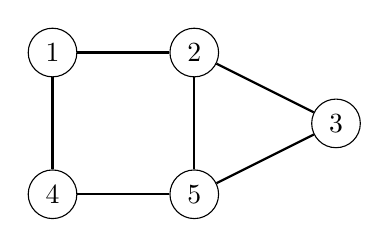
\begin{tikzpicture}[scale=0.9]
\node[draw, circle] (1) at (1,5) {$1$};
\node[draw, circle] (2) at (3,5) {$2$};
\node[draw, circle] (3) at (5,4) {$3$};
\node[draw, circle] (4) at (1,3) {$4$};
\node[draw, circle] (5) at (3,3) {$5$};

\path[draw,thick,-] (1) -- (2);
\path[draw,thick,-] (2) -- (3);
\path[draw,thick,-] (1) -- (4);
\path[draw,thick,-] (3) -- (5);
\path[draw,thick,-] (2) -- (5);
\path[draw,thick,-] (4) -- (5);
\end{tikzpicture}
\end{center}
tem um caminho Euleriano do nó 2 ao nó 5:
\begin{center}
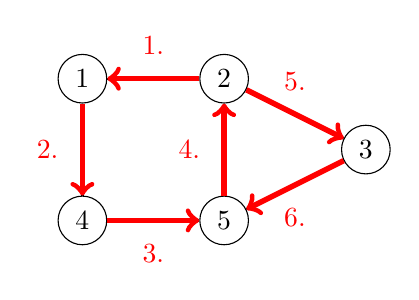
\begin{tikzpicture}[scale=0.9]
\node[draw, circle] (1) at (1,5) {$1$};
\node[draw, circle] (2) at (3,5) {$2$};
\node[draw, circle] (3) at (5,4) {$3$};
\node[draw, circle] (4) at (1,3) {$4$};
\node[draw, circle] (5) at (3,3) {$5$};

\path[draw,thick,-] (1) -- (2);
\path[draw,thick,-] (2) -- (3);
\path[draw,thick,-] (1) -- (4);
\path[draw,thick,-] (3) -- (5);
\path[draw,thick,-] (2) -- (5);
\path[draw,thick,-] (4) -- (5);

\path[draw=red,thick,->,line width=2pt] (2) -- node[font=\small,label={[red]north:1.}] {} (1);
\path[draw=red,thick,->,line width=2pt] (1) -- node[font=\small,label={[red]left:2.}] {} (4);
\path[draw=red,thick,->,line width=2pt] (4) -- node[font=\small,label={[red]south:3.}] {} (5);
\path[draw=red,thick,->,line width=2pt] (5) -- node[font=\small,label={[red]left:4.}] {} (2);
\path[draw=red,thick,->,line width=2pt] (2) -- node[font=\small,label={[red]north:5.}] {} (3);
\path[draw=red,thick,->,line width=2pt] (3) -- node[font=\small,label={[red]south:6.}] {} (5);
\end{tikzpicture}
\end{center}
\index{Eulerian circuit}
Um \key{circuito Euleriano}
é um caminho Euleriano que começa e termina
no mesmo nó.
Por exemplo, o grafo
\begin{center}
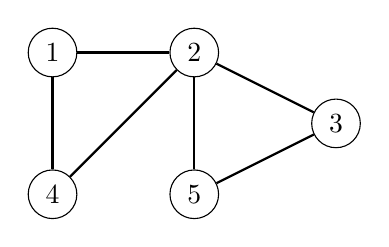
\begin{tikzpicture}[scale=0.9]
\node[draw, circle] (1) at (1,5) {$1$};
\node[draw, circle] (2) at (3,5) {$2$};
\node[draw, circle] (3) at (5,4) {$3$};
\node[draw, circle] (4) at (1,3) {$4$};
\node[draw, circle] (5) at (3,3) {$5$};

\path[draw,thick,-] (1) -- (2);
\path[draw,thick,-] (2) -- (3);
\path[draw,thick,-] (1) -- (4);
\path[draw,thick,-] (3) -- (5);
\path[draw,thick,-] (2) -- (5);
\path[draw,thick,-] (2) -- (4);
\end{tikzpicture}
\end{center}
possui um circuito Euleriano que começa e termina no nó 1:
\begin{center}
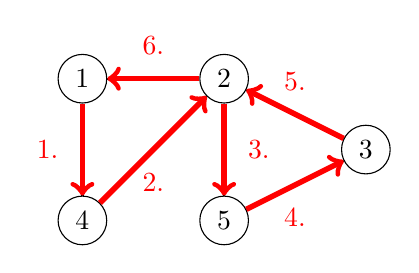
\begin{tikzpicture}[scale=0.9]
\node[draw, circle] (1) at (1,5) {$1$};
\node[draw, circle] (2) at (3,5) {$2$};
\node[draw, circle] (3) at (5,4) {$3$};
\node[draw, circle] (4) at (1,3) {$4$};
\node[draw, circle] (5) at (3,3) {$5$};

\path[draw,thick,-] (1) -- (2);
\path[draw,thick,-] (2) -- (3);
\path[draw,thick,-] (1) -- (4);
\path[draw,thick,-] (3) -- (5);
\path[draw,thick,-] (2) -- (5);
\path[draw,thick,-] (2) -- (4);

\path[draw=red,thick,->,line width=2pt] (1) -- node[font=\small,label={[red]left:1.}] {} (4);
\path[draw=red,thick,->,line width=2pt] (4) -- node[font=\small,label={[red]south:2.}] {} (2);
\path[draw=red,thick,->,line width=2pt] (2) -- node[font=\small,label={[red]right:3.}] {} (5);
\path[draw=red,thick,->,line width=2pt] (5) -- node[font=\small,label={[red]south:4.}] {} (3);
\path[draw=red,thick,->,line width=2pt] (3) -- node[font=\small,label={[red]north:5.}] {} (2);
\path[draw=red,thick,->,line width=2pt] (2) -- node[font=\small,label={[red]north:6.}] {} (1);
\end{tikzpicture}
\end{center}

\subsubsection{Existência}

A existência de caminhos e circuitos Eulerianos
depende dos graus dos nós.
Primeiro, um grafo não direcionado tem um caminho Euleriano
exatamente quando todas as arestas
pertencem ao mesmo componente conexo e
\begin{itemize}
\item o grau de cada nó é par \emph{ou}
\item o grau de exatamente dois nós é ímpar,
e o grau de todos os outros nós é par.
\end{itemize}

No primeiro caso, cada caminho Euleriano também é um circuito Euleriano.
No segundo caso, os nós de grau ímpar são os nós inicial
e final de um caminho Euleriano que não é um circuito Euleriano.

\begin{samepage}
Por exemplo, no grafo
\begin{center}
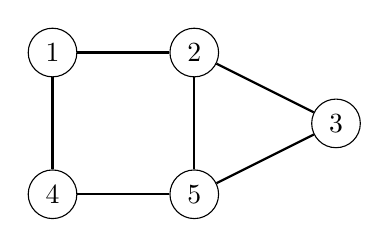
\begin{tikzpicture}[scale=0.9]
\node[draw, circle] (1) at (1,5) {$1$};
\node[draw, circle] (2) at (3,5) {$2$};
\node[draw, circle] (3) at (5,4) {$3$};
\node[draw, circle] (4) at (1,3) {$4$};
\node[draw, circle] (5) at (3,3) {$5$};

\path[draw,thick,-] (1) -- (2);
\path[draw,thick,-] (2) -- (3);
\path[draw,thick,-] (1) -- (4);
\path[draw,thick,-] (3) -- (5);
\path[draw,thick,-] (2) -- (5);
\path[draw,thick,-] (4) -- (5);
\end{tikzpicture}
\end{center}
\end{samepage}
os nós 1, 3 e 4 têm grau 2,
e os nós 2 e 5 têm grau 3.
Exatamente dois nós têm grau ímpar,
então há um caminho Euleriano entre os nós 2 e 5,
mas o grafo não contém um circuito Euleriano.

Em um grafo direcionado,
focamos nos graus de entrada e saída
dos nós.
Um grafo direcionado contém um caminho Euleriano
exatamente quando todas as arestas pertencem ao mesmo
componente conexo e
\begin{itemize}
\item em cada nó, o grau de entrada é igual ao grau de saída, \emph{ou}
\item em um nó, o grau de entrada é um a mais que o grau de saída,
em outro nó, o grau de saída é um a mais que o grau de entrada,
e em todos os outros nós, o grau de entrada é igual ao grau de saída.
\end{itemize}

No primeiro caso, cada caminho Euleriano
também é um circuito Euleriano,
e no segundo caso, o grafo contém um caminho Euleriano
que começa no nó cujo grau de saída é maior
e termina no nó cujo grau de entrada é maior.

Por exemplo, no grafo
\begin{center}
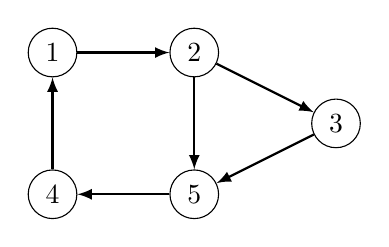
\begin{tikzpicture}[scale=0.9]
\node[draw, circle] (1) at (1,5) {$1$};
\node[draw, circle] (2) at (3,5) {$2$};
\node[draw, circle] (3) at (5,4) {$3$};
\node[draw, circle] (4) at (1,3) {$4$};
\node[draw, circle] (5) at (3,3) {$5$};

\path[draw,thick,->,>=latex] (1) -- (2);
\path[draw,thick,->,>=latex] (2) -- (3);
\path[draw,thick,->,>=latex] (4) -- (1);
\path[draw,thick,->,>=latex] (3) -- (5);
\path[draw,thick,->,>=latex] (2) -- (5);
\path[draw,thick,->,>=latex] (5) -- (4);
\end{tikzpicture}
\end{center}
os nós 1, 3 e 4 têm grau de entrada 1 e grau de saída 1,
o nó 2 tem grau de entrada 1 e grau de saída 2,
e o nó 5 tem grau de entrada 2 e grau de saída 1.
Portanto, o grafo contém um caminho Euleriano
do nó 2 ao nó 5:
\begin{center}
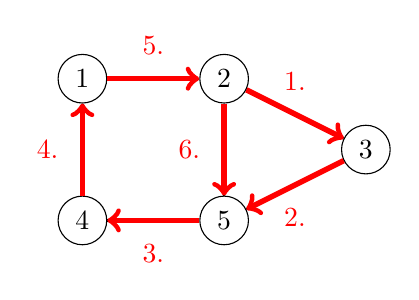
\begin{tikzpicture}[scale=0.9]
\node[draw, circle] (1) at (1,5) {$1$};
\node[draw, circle] (2) at (3,5) {$2$};
\node[draw, circle] (3) at (5,4) {$3$};
\node[draw, circle] (4) at (1,3) {$4$};
\node[draw, circle] (5) at (3,3) {$5$};

\path[draw,thick,-] (1) -- (2);
\path[draw,thick,-] (2) -- (3);
\path[draw,thick,-] (1) -- (4);
\path[draw,thick,-] (3) -- (5);
\path[draw,thick,-] (2) -- (5);
\path[draw,thick,-] (4) -- (5);

\path[draw=red,thick,->,line width=2pt] (2) -- node[font=\small,label={[red]north:1.}] {} (3);
\path[draw=red,thick,->,line width=2pt] (3) -- node[font=\small,label={[red]south:2.}] {} (5);
\path[draw=red,thick,->,line width=2pt] (5) -- node[font=\small,label={[red]south:3.}] {} (4);
\path[draw=red,thick,->,line width=2pt] (4) -- node[font=\small,label={[red]left:4.}] {} (1);
\path[draw=red,thick,->,line width=2pt] (1) -- node[font=\small,label={[red]north:5.}] {} (2);
\path[draw=red,thick,->,line width=2pt] (2) -- node[font=\small,label={[red]left:6.}] {} (5);
\end{tikzpicture}
\end{center}

\subsubsection{Algoritmo de Hierholzer}

\index{Hierholzer's algorithm}

\key{O algoritmo de Hierholzer}\footnote{O algoritmo foi publicado
em 1873 após a morte de Hierholzer \cite{hie73}.} é um método eficiente para construir
um circuito Euleriano.
O algoritmo consiste em várias rodadas,
cada uma das quais adiciona novas arestas ao circuito.
Claro, assumimos que o grafo contém
um circuito Euleriano; caso contrário, o algoritmo de Hierholzer
não pode encontrá-lo.

Primeiro, o algoritmo constrói um circuito que contém
algumas (não necessariamente todas) das arestas do grafo.
Depois disso, o algoritmo estende o circuito
passo a passo adicionando subcircuitos a ele.
O processo continua até que todas as arestas tenham sido adicionadas
ao circuito.

O algoritmo estende o circuito sempre encontrando
um nó $x$ que pertence ao circuito, mas tem
uma aresta de saída que não está incluída no circuito.
O algoritmo constrói um novo caminho a partir do nó $x$
que contém apenas arestas que ainda não estão no circuito.
Cedo ou tarde,
o caminho retornará ao nó $x$,
o que cria um subcircuito.

Se o grafo contiver apenas um caminho Euleriano,
ainda podemos usar o algoritmo de Hierholzer
para encontrá-lo adicionando uma aresta extra ao grafo
e removendo a aresta após o circuito
ter sido construído.
Por exemplo, em um grafo não direcionado,
adicionamos a aresta extra entre os dois
nós de grau ímpar.

A seguir, veremos como o algoritmo de Hierholzer
constrói um circuito Euleriano para um grafo não direcionado.

\subsubsection{Exemplo}

\begin{samepage}
Vamos considerar o seguinte grafo:
\begin{center}
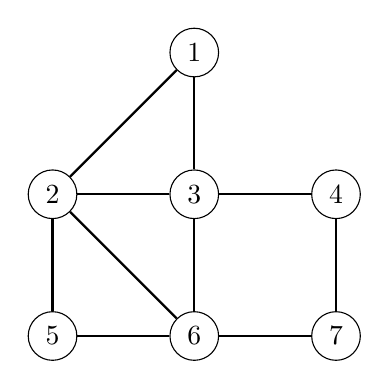
\begin{tikzpicture}[scale=0.9]
\node[draw, circle] (1) at (3,5) {$1$};
\node[draw, circle] (2) at (1,3) {$2$};
\node[draw, circle] (3) at (3,3) {$3$};
\node[draw, circle] (4) at (5,3) {$4$};
\node[draw, circle] (5) at (1,1) {$5$};
\node[draw, circle] (6) at (3,1) {$6$};
\node[draw, circle] (7) at (5,1) {$7$};

\path[draw,thick,-] (1) -- (2);
\path[draw,thick,-] (1) -- (3);
\path[draw,thick,-] (2) -- (3);
\path[draw,thick,-] (2) -- (5);
\path[draw,thick,-] (2) -- (6);
\path[draw,thick,-] (3) -- (4);
\path[draw,thick,-] (3) -- (6);
\path[draw,thick,-] (4) -- (7);
\path[draw,thick,-] (5) -- (6);
\path[draw,thick,-] (6) -- (7);
\end{tikzpicture}
\end{center}
\end{samepage}

\begin{samepage}
Suponha que o algoritmo primeiro cria um circuito
que começa no nó 1.
Um circuito possível é
$1 \rightarrow 2 \rightarrow 3 \rightarrow 1$:
\begin{center}
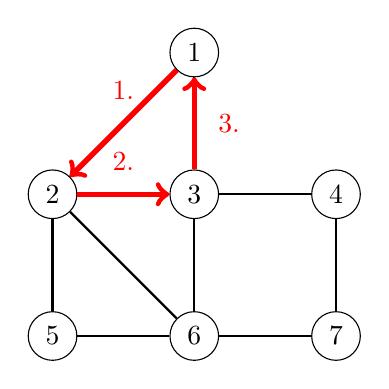
\begin{tikzpicture}[scale=0.9]
\node[draw, circle] (1) at (3,5) {$1$};
\node[draw, circle] (2) at (1,3) {$2$};
\node[draw, circle] (3) at (3,3) {$3$};
\node[draw, circle] (4) at (5,3) {$4$};
\node[draw, circle] (5) at (1,1) {$5$};
\node[draw, circle] (6) at (3,1) {$6$};
\node[draw, circle] (7) at (5,1) {$7$};

\path[draw,thick,-] (1) -- (2);
\path[draw,thick,-] (1) -- (3);
\path[draw,thick,-] (2) -- (3);
\path[draw,thick,-] (2) -- (5);
\path[draw,thick,-] (2) -- (6);
\path[draw,thick,-] (3) -- (4);
\path[draw,thick,-] (3) -- (6);
\path[draw,thick,-] (4) -- (7);
\path[draw,thick,-] (5) -- (6);
\path[draw,thick,-] (6) -- (7);

\path[draw=red,thick,->,line width=2pt] (1) -- node[font=\small,label={[red]north:1.}] {} (2);
\path[draw=red,thick,->,line width=2pt] (2) -- node[font=\small,label={[red]north:2.}] {} (3);
\path[draw=red,thick,->,line width=2pt] (3) -- node[font=\small,label={[red]east:3.}] {} (1);
\end{tikzpicture}
\end{center}
\end{samepage}
Depois disso, o algoritmo adiciona
o subcircuito
$2 \rightarrow 5 \rightarrow 6 \rightarrow 2$
ao circuito:
\begin{center}
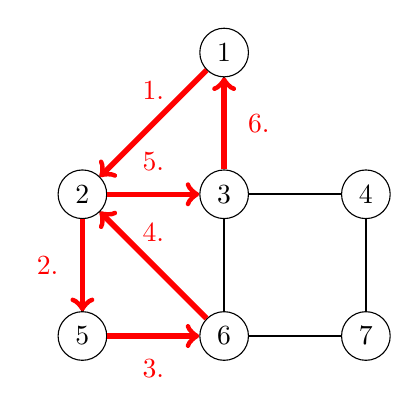
\begin{tikzpicture}[scale=0.9]
\node[draw, circle] (1) at (3,5) {$1$};
\node[draw, circle] (2) at (1,3) {$2$};
\node[draw, circle] (3) at (3,3) {$3$};
\node[draw, circle] (4) at (5,3) {$4$};
\node[draw, circle] (5) at (1,1) {$5$};
\node[draw, circle] (6) at (3,1) {$6$};
\node[draw, circle] (7) at (5,1) {$7$};

\path[draw,thick,-] (1) -- (2);
\path[draw,thick,-] (1) -- (3);
\path[draw,thick,-] (2) -- (3);
\path[draw,thick,-] (2) -- (5);
\path[draw,thick,-] (2) -- (6);
\path[draw,thick,-] (3) -- (4);
\path[draw,thick,-] (3) -- (6);
\path[draw,thick,-] (4) -- (7);
\path[draw,thick,-] (5) -- (6);
\path[draw,thick,-] (6) -- (7);

\path[draw=red,thick,->,line width=2pt] (1) -- node[font=\small,label={[red]north:1.}] {} (2);
\path[draw=red,thick,->,line width=2pt] (2) -- node[font=\small,label={[red]west:2.}] {} (5);
\path[draw=red,thick,->,line width=2pt] (5) -- node[font=\small,label={[red]south:3.}] {} (6);
\path[draw=red,thick,->,line width=2pt] (6) -- node[font=\small,label={[red]north:4.}] {} (2);
\path[draw=red,thick,->,line width=2pt] (2) -- node[font=\small,label={[red]north:5.}] {} (3);
\path[draw=red,thick,->,line width=2pt] (3) -- node[font=\small,label={[red]east:6.}] {} (1);
\end{tikzpicture}
\end{center}
Finalmente, o algoritmo adiciona o subcircuito
$6 \rightarrow 3 \rightarrow 4 \rightarrow 7 \rightarrow 6$
ao circuito:
\begin{center}
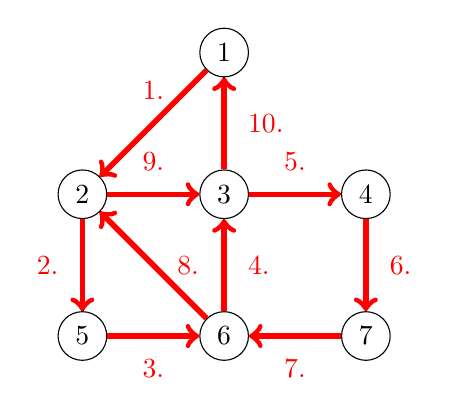
\begin{tikzpicture}[scale=0.9]
\node[draw, circle] (1) at (3,5) {$1$};
\node[draw, circle] (2) at (1,3) {$2$};
\node[draw, circle] (3) at (3,3) {$3$};
\node[draw, circle] (4) at (5,3) {$4$};
\node[draw, circle] (5) at (1,1) {$5$};
\node[draw, circle] (6) at (3,1) {$6$};
\node[draw, circle] (7) at (5,1) {$7$};

\path[draw,thick,-] (1) -- (2);
\path[draw,thick,-] (1) -- (3);
\path[draw,thick,-] (2) -- (3);
\path[draw,thick,-] (2) -- (5);
\path[draw,thick,-] (2) -- (6);
\path[draw,thick,-] (3) -- (4);
\path[draw,thick,-] (3) -- (6);
\path[draw,thick,-] (4) -- (7);
\path[draw,thick,-] (5) -- (6);
\path[draw,thick,-] (6) -- (7);

\path[draw=red,thick,->,line width=2pt] (1) -- node[font=\small,label={[red]north:1.}] {} (2);
\path[draw=red,thick,->,line width=2pt] (2) -- node[font=\small,label={[red]west:2.}] {} (5);
\path[draw=red,thick,->,line width=2pt] (5) -- node[font=\small,label={[red]south:3.}] {} (6);
\path[draw=red,thick,->,line width=2pt] (6) -- node[font=\small,label={[red]east:4.}] {} (3);
\path[draw=red,thick,->,line width=2pt] (3) -- node[font=\small,label={[red]north:5.}] {} (4);
\path[draw=red,thick,->,line width=2pt] (4) -- node[font=\small,label={[red]east:6.}] {} (7);
\path[draw=red,thick,->,line width=2pt] (7) -- node[font=\small,label={[red]south:7.}] {} (6);
\path[draw=red,thick,->,line width=2pt] (6) -- node[font=\small,label={[red]right:8.}] {} (2);
\path[draw=red,thick,->,line width=2pt] (2) -- node[font=\small,label={[red]north:9.}] {} (3);
\path[draw=red,thick,->,line width=2pt] (3) -- node[font=\small,label={[red]east:10.}] {} (1);
\end{tikzpicture}
\end{center}
Agora todas as arestas estão incluídas no circuito,
então construímos com sucesso um circuito Euleriano.

\section{Caminhos Hamiltonianos}

\index{Hamiltonian path}

Um \key{caminho Hamiltoniano}
%\footnote{W. R. Hamilton (1805--1865) foi um matemático irlandês.}
é um caminho
que visita cada nó do grafo exatamente uma vez.
Por exemplo, o grafo
\begin{center}
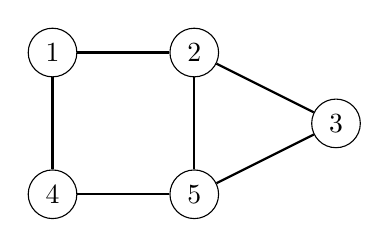
\begin{tikzpicture}[scale=0.9]
\node[draw, circle] (1) at (1,5) {$1$};
\node[draw, circle] (2) at (3,5) {$2$};
\node[draw, circle] (3) at (5,4) {$3$};
\node[draw, circle] (4) at (1,3) {$4$};
\node[draw, circle] (5) at (3,3) {$5$};

\path[draw,thick,-] (1) -- (2);
\path[draw,thick,-] (2) -- (3);
\path[draw,thick,-] (1) -- (4);
\path[draw,thick,-] (3) -- (5);
\path[draw,thick,-] (2) -- (5);
\path[draw,thick,-] (4) -- (5);
\end{tikzpicture}
\end{center}
contém um caminho Hamiltoniano do nó 1 ao nó 3:
\begin{center}
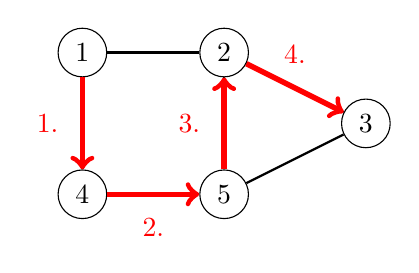
\begin{tikzpicture}[scale=0.9]
\node[draw, circle] (1) at (1,5) {$1$};
\node[draw, circle] (2) at (3,5) {$2$};
\node[draw, circle] (3) at (5,4) {$3$};
\node[draw, circle] (4) at (1,3) {$4$};
\node[draw, circle] (5) at (3,3) {$5$};

\path[draw,thick,-] (1) -- (2);
\path[draw,thick,-] (2) -- (3);
\path[draw,thick,-] (1) -- (4);
\path[draw,thick,-] (3) -- (5);
\path[draw,thick,-] (2) -- (5);
\path[draw,thick,-] (4) -- (5);

\path[draw=red,thick,->,line width=2pt] (1) -- node[font=\small,label={[red]left:1.}] {} (4);
\path[draw=red,thick,->,line width=2pt] (4) -- node[font=\small,label={[red]south:2.}] {} (5);
\path[draw=red,thick,->,line width=2pt] (5) -- node[font=\small,label={[red]left:3.}] {} (2);
\path[draw=red,thick,->,line width=2pt] (2) -- node[font=\small,label={[red]north:4.}] {} (3);
\end{tikzpicture}
\end{center}

\index{Hamiltonian circuit}

Se um caminho Hamiltoniano começa e termina no mesmo nó,
ele é chamado de \key{circuito Hamiltoniano}.
O grafo acima também possui um circuito Hamiltoniano
que começa e termina no nó 1:
\begin{center}
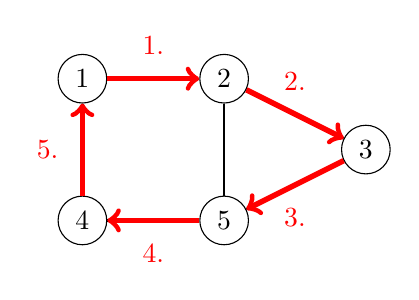
\begin{tikzpicture}[scale=0.9]
\node[draw, circle] (1) at (1,5) {$1$};
\node[draw, circle] (2) at (3,5) {$2$};
\node[draw, circle] (3) at (5,4) {$3$};
\node[draw, circle] (4) at (1,3) {$4$};
\node[draw, circle] (5) at (3,3) {$5$};

\path[draw,thick,-] (1) -- (2);
\path[draw,thick,-] (2) -- (3);
\path[draw,thick,-] (1) -- (4);
\path[draw,thick,-] (3) -- (5);
\path[draw,thick,-] (2) -- (5);
\path[draw,thick,-] (4) -- (5);

\path[draw=red,thick,->,line width=2pt] (1) -- node[font=\small,label={[red]north:1.}] {} (2);
\path[draw=red,thick,->,line width=2pt] (2) -- node[font=\small,label={[red]north:2.}] {} (3);
\path[draw=red,thick,->,line width=2pt] (3) -- node[font=\small,label={[red]south:3.}] {} (5);
\path[draw=red,thick,->,line width=2pt] (5) -- node[font=\small,label={[red]south:4.}] {} (4);
\path[draw=red,thick,->,line width=2pt] (4) -- node[font=\small,label={[red]left:5.}] {} (1);
\end{tikzpicture}
\end{center}

\subsubsection{Existência}

Nenhum método eficiente é conhecido para testar se um grafo
contém um caminho Hamiltoniano, e o problema é NP-difícil.
Ainda assim, em alguns casos especiais, podemos ter certeza
de que um grafo contém um caminho Hamiltoniano.

Uma observação simples é que se o grafo for completo,
ou seja, há uma aresta entre todos os pares de nós,
ele também contém um caminho Hamiltoniano.
Resultados ainda mais fortes foram alcançados:

\begin{itemize}
\item
\index{Dirac's theorem}
\key{Teorema de Dirac}: %\cite{dir52}
Se o grau de cada nó for pelo menos $n/2$,
o grafo contém um caminho Hamiltoniano.
\item
\index{Ore's theorem}
\key{Teorema de Ore}: %\cite{ore60}
Se a soma dos graus de cada par de nós não adjacentes
for pelo menos $n$,
o grafo contém um caminho Hamiltoniano.
\end{itemize}

Uma propriedade comum nesses teoremas e outros resultados é
que eles garantem a existência de um caminho Hamiltoniano
se o grafo tiver \emph{um grande número} de arestas.
Isso faz sentido, porque quanto mais arestas o grafo contiver,
mais possibilidades existem para construir um caminho Hamiltoniano.

\subsubsection{Construção}

Como não há como verificar eficientemente se um Hamiltoniano
caminho existe, é claro que também não há método
para construir o caminho de forma eficiente, porque caso contrário
poderíamos apenas tentar construir o caminho e ver
se ele existe.

Uma maneira simples de procurar um caminho Hamiltoniano é
usar um algoritmo de backtracking que percorre todas
as maneiras possíveis de construir o caminho.
A complexidade de tempo de tal algoritmo é pelo menos $O(n!)$,
porque existem $n!$ maneiras diferentes de escolher a ordem de $n$ nós.

Uma solução mais eficiente é baseada em programação dinâmica
(ver Capítulo 10.5).
A ideia é calcular valores
de uma função $\texttt{possível}(S,x)$,
onde $S$ é um subconjunto de nós e $x$
é um dos nós.
A função indica se há um caminho Hamiltoniano
que visita os nós de $S$ e termina no nó $x$.
É possível implementar esta solução em tempo $O(2^n n^2)$.

\section{Sequências de De Bruijn}

\index{De Bruijn sequence}

Uma \key{sequência de De Bruijn}
é uma string que contém
cada string de comprimento $n$
exatamente uma vez como uma substring, para um
alfabeto fixo de $k$ caracteres.
O comprimento de tal string é
$k^n+n-1$ caracteres.
Por exemplo, quando $n=3$ e $k=2$,
um exemplo de uma sequência de De Bruijn é
\[0001011100.\]
As substrings desta string são todas
combinações de três bits:
000, 001, 010, 011, 100, 101, 110 e 111.

Acontece que cada sequência de De Bruijn
corresponde a um caminho Euleriano em um grafo.
A ideia é construir um grafo onde
cada nó contém uma string de $n-1$ caracteres
e cada aresta adiciona um caractere à string.
O seguinte grafo corresponde ao cenário acima:

\begin{center}
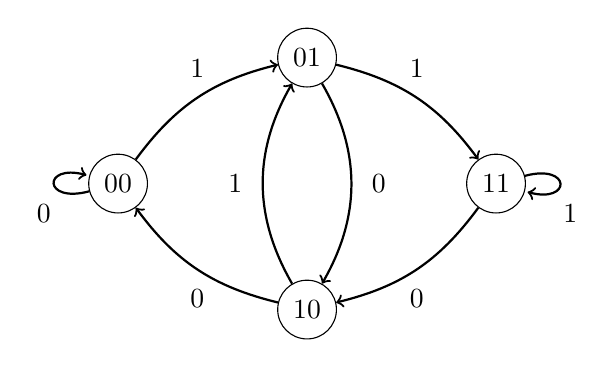
\begin{tikzpicture}[scale=0.8]
\node[draw, circle] (00) at (-3,0) {00};
\node[draw, circle] (11) at (3,0) {11};
\node[draw, circle] (01) at (0,2) {01};
\node[draw, circle] (10) at (0,-2) {10};

\path[draw,thick,->] (00) edge [bend left=20] node[font=\small,label=1] {} (01);
\path[draw,thick,->] (01) edge [bend left=20] node[font=\small,label=1] {} (11);
\path[draw,thick,->] (11) edge [bend left=20] node[font=\small,label=below:0] {} (10);
\path[draw,thick,->] (10) edge [bend left=20] node[font=\small,label=below:0] {} (00);

\path[draw,thick,->] (01) edge [bend left=30] node[font=\small,label=right:0] {} (10);
\path[draw,thick,->] (10) edge [bend left=30] node[font=\small,label=left:1] {} (01);

\path[draw,thick,-] (00) edge [loop left] node[font=\small,label=below:0] {} (00);
\path[draw,thick,-] (11) edge [loop right] node[font=\small,label=below:1] {} (11);
\end{tikzpicture}
\end{center}

Um caminho Euleriano neste grafo corresponde a uma string
que contém todas as strings de comprimento $n$.
A string contém os caracteres do nó inicial
e todos os caracteres das arestas.
O nó inicial tem $n-1$ caracteres
e há $k^n$ caracteres nas arestas,
então o comprimento da string é $k^n+n-1$.

\section{Passeio do Cavalo}

\index{knight's tour}

Um \key{passeio do cavalo} é uma sequência de movimentos
de um cavalo em um tabuleiro de xadrez $n \times n$
seguindo as regras do xadrez, de forma que o cavalo
visite cada casa exatamente uma vez.
Um passeio do cavalo é chamado de \emph{passeio fechado}
se o cavalo finalmente retorna à casa inicial e
caso contrário, é chamado de \emph{passeio aberto}.

Por exemplo, aqui está um passeio do cavalo aberto em um tabuleiro $5 \times 5$:

\begin{center}
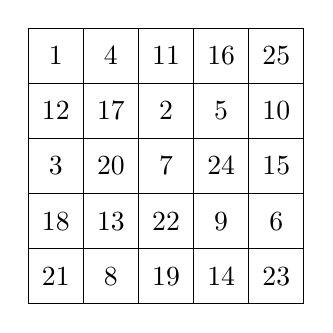
\begin{tikzpicture}[scale=0.7]
\draw (0,0) grid (5,5);
\node at (0.5,4.5) {$1$};
\node at (1.5,4.5) {$4$};
\node at (2.5,4.5) {$11$};
\node at (3.5,4.5) {$16$};
\node at (4.5,4.5) {$25$};
\node at (0.5,3.5) {$12$};
\node at (1.5,3.5) {$17$};
\node at (2.5,3.5) {$2$};
\node at (3.5,3.5) {$5$};
\node at (4.5,3.5) {$10$};
\node at (0.5,2.5) {$3$};
\node at (1.5,2.5) {$20$};
\node at (2.5,2.5) {$7$};
\node at (3.5,2.5) {$24$};
\node at (4.5,2.5) {$15$};
\node at (0.5,1.5) {$18$};
\node at (1.5,1.5) {$13$};
\node at (2.5,1.5) {$22$};
\node at (3.5,1.5) {$9$};
\node at (4.5,1.5) {$6$};
\node at (0.5,0.5) {$21$};
\node at (1.5,0.5) {$8$};
\node at (2.5,0.5) {$19$};
\node at (3.5,0.5) {$14$};
\node at (4.5,0.5) {$23$};
\end{tikzpicture}
\end{center}

Um passeio do cavalo corresponde a um caminho Hamiltoniano em um grafo
cujos nós representam as casas do tabuleiro,
e dois nós são conectados com uma aresta se um cavalo
pode se mover entre as casas de acordo com as regras do xadrez.

Uma maneira natural de construir um passeio do cavalo é usar o algoritmo de backtracking.
A busca pode ser mais eficiente usando
\emph{heurísticas} que tentam guiar o cavalo para que
um passeio completo seja encontrado rapidamente.

\subsubsection{Regra de Warnsdorf}

\index{heuristic}
\index{Warnsdorf's rule}

\key{A regra de Warnsdorf} é uma heurística simples e eficaz
para encontrar um passeio do cavalo\footnote{Essa heurística foi proposta
no livro de Warnsdorf \cite{war23} em 1823. Existem
também algoritmos polinomiais para encontrar passeios do cavalo
\cite{par97}, mas eles são mais complicados.}.
Usando a regra, é possível construir um passeio de forma eficiente
mesmo em um tabuleiro grande.
A ideia é mover o cavalo sempre para que ele termine
em uma casa onde o número de movimentos possíveis seja o mais
\emph{pequeno} possível.

Por exemplo, na seguinte situação, existem cinco
casas possíveis para as quais o cavalo pode se mover (casas $a \ldots e$):
\begin{center}
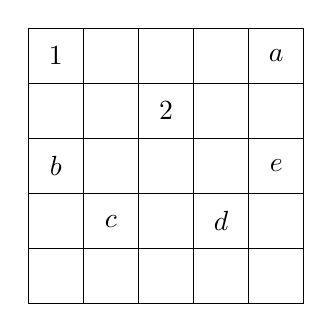
\begin{tikzpicture}[scale=0.7]
\draw (0,0) grid (5,5);
\node at (0.5,4.5) {$1$};
\node at (2.5,3.5) {$2$};
\node at (4.5,4.5) {$a$};
\node at (0.5,2.5) {$b$};
\node at (4.5,2.5) {$e$};
\node at (1.5,1.5) {$c$};
\node at (3.5,1.5) {$d$};
\end{tikzpicture}
\end{center}
Nesta situação, a regra de Warnsdorf move o cavalo para a casa $a$,
porque após esta escolha, há apenas um único movimento possível.
As outras escolhas moveriam o cavalo para casas onde
haveria três movimentos disponíveis.


